\subsection{Topology Calculations}
In an effort to provide better fidelity of the mars topology, a benchmark calculation was 
designed that consisted of adding mountains and craters to the Mars surface. 
The input files were created in FLUKA and run similarly to the benchmark calculations 
for the atmospheres. 

\subsection*{Geometry}
The mountains were created on the surface of Mars and were designed to be 5 km high 
and 10 km wide, where as the craters were designed to be 5 km deep and 10 km wide. 
Variations of the mountain and crater described above were modeled. Nine different 
models were created for mountains and nine for craters. 
These variations were 1/3, 2/3 and 3/3 of the height with base of 1/3, 2/3 and 3/3. 

In the interest of calculating dose, detectors were set at the top, half way up, base, 
and away from the mountain. The crater had similar detectors. A schematics of the set up 
can be seen in figure \ref{setup_mountain} for mountains and 
figure \ref{setup_crater} for craters.

\begin{figure}[h]
\centering
\begin{subfigure}[b]{.45\textwidth}
\frame{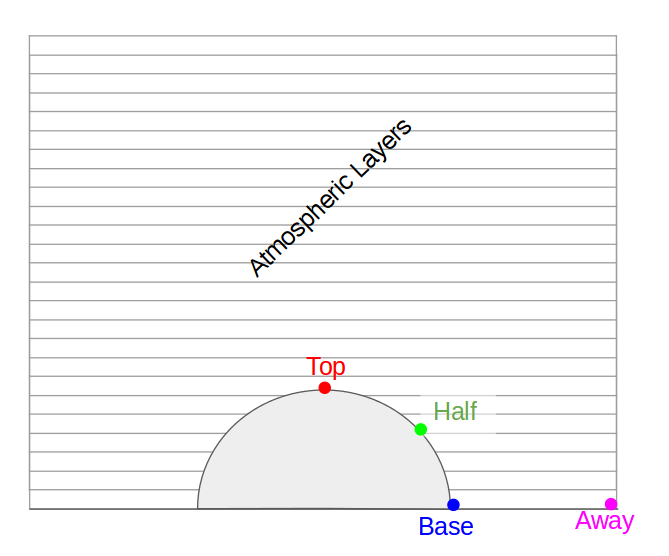
\includegraphics[width=0.85\linewidth,height=5cm]{../figs/mountain.png}}
\caption{Mountain}
\label{setup_mountain}
\end{subfigure}
%
\hspace{0.10cm}
%
\begin{subfigure}[b]{.4\textwidth}
\centering
\frame{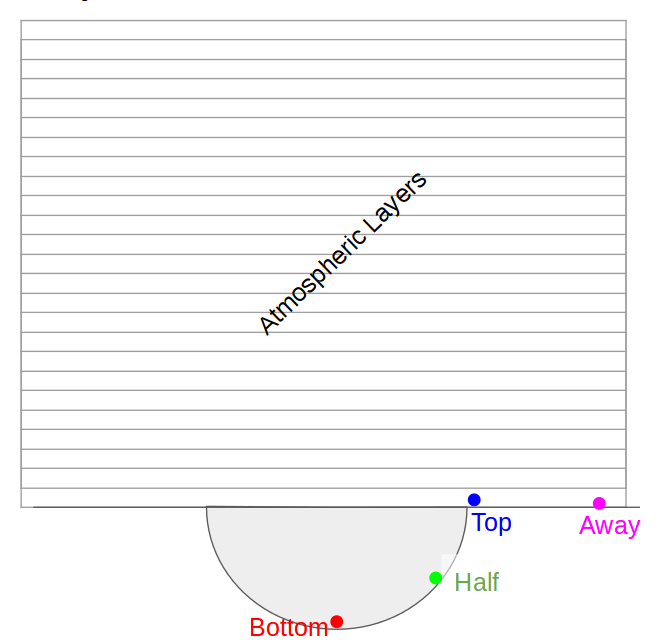
\includegraphics[width=.85\linewidth,height=5cm]{../figs/crater.png}}
\caption{Crater}
\label{setup_crater}
\end{subfigure}
\caption{Geometry set up with detectors and atmospheric layers}
\end{figure}


\subsection*{Results}
A mountain and a crater with base of 10 km and height or depth of 5 km were used to 
obtain the following results. 

For the first calculation tallies for energy deposition were set and the results can be seen 
in figure \ref{energy_mountain} for mountains and in figure \ref{energy_crater} 
for craters. 

\begin{figure}
 \begin{centering}
 \centering
 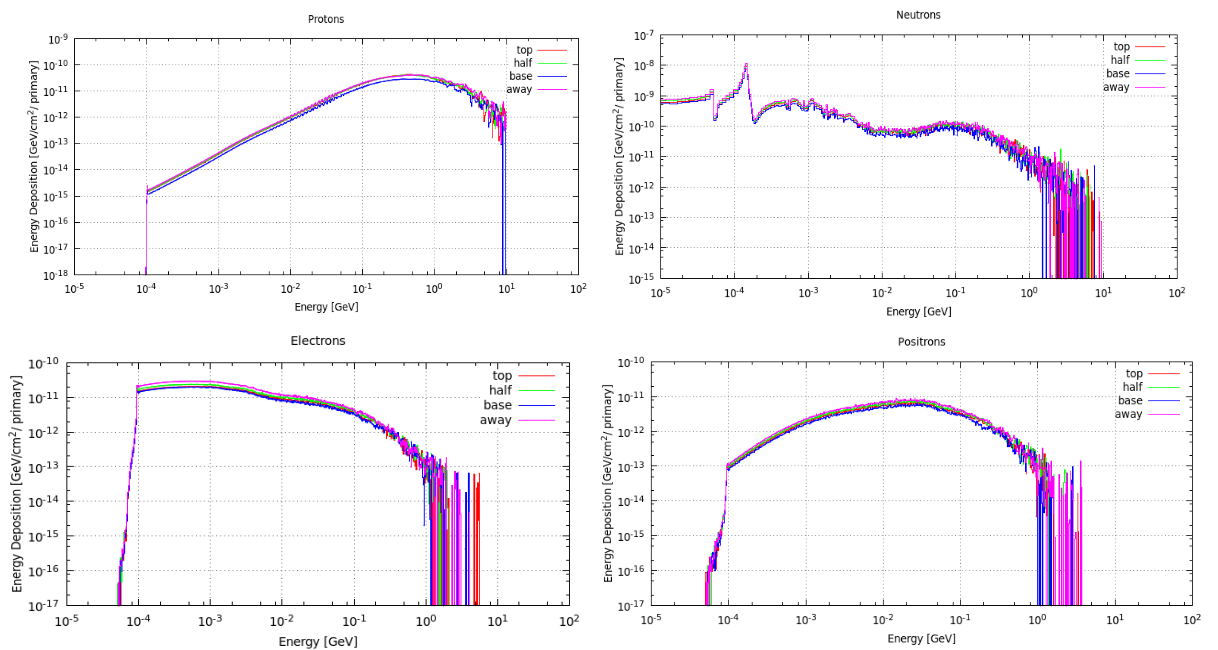
\includegraphics[width=0.6\linewidth,height=7cm]{../figs/energy_deposition_mountain.png}
 \caption{Energy deposition in the mountain for protons, neutrons, electrons and positrons}
 \label{energy_mountain}
 \end{centering}
\end{figure}

\begin{figure}
 \begin{centering}
 \centering
 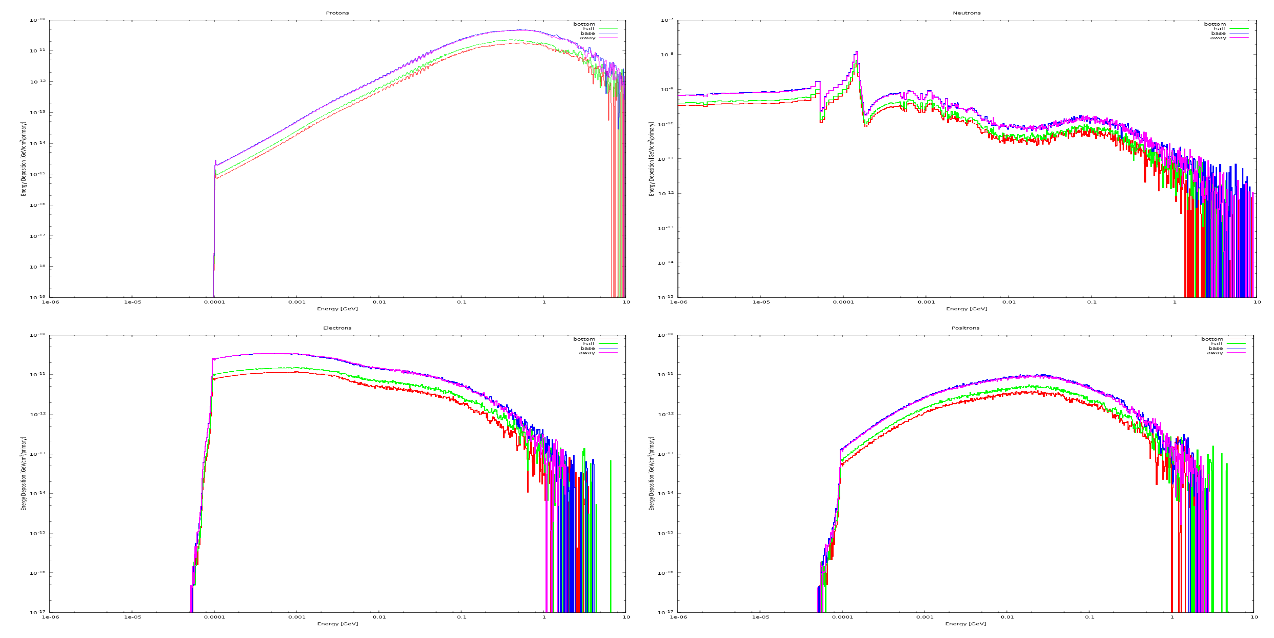
\includegraphics[width=0.6\linewidth,height=7cm]{../figs/deposition_crater.png}
 \caption{Energy deposition in the crater for protons, neutrons, electrons and positrons}
 \label{energy_crater}
 \end{centering}
\end{figure}

The total reponse at each of the detectors was also calculated for several particles 
of interest. The results can be seen in figure \ref{response_mountain} and \ref{response_crater}.

\begin{figure}
\centering
\begin{subfigure}[b]{.45\textwidth}
\frame{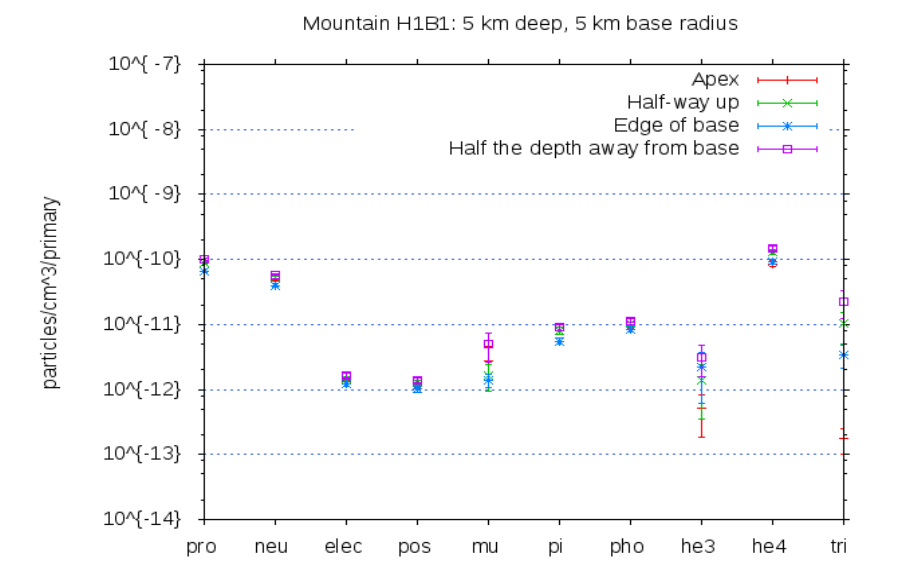
\includegraphics[width=0.85\linewidth,height=5cm]{../figs/mountain_response.png}}
\caption{Mountain}
\label{response_mountain}
\end{subfigure}
%
\hspace{0.10cm}
%
\begin{subfigure}[b]{.4\textwidth}
\centering
\frame{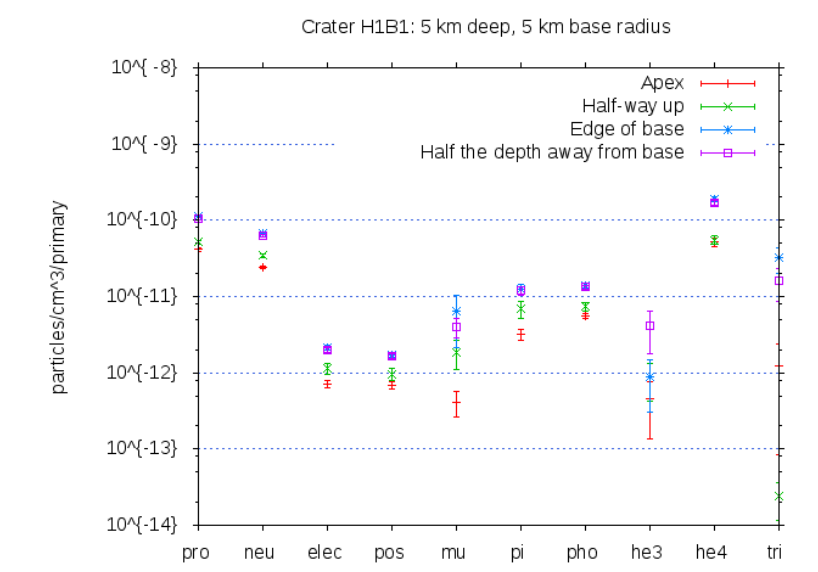
\includegraphics[width=.85\linewidth,height=5cm]{../figs/crater_response.png}}
\caption{Crater}
\label{response_crater}
\end{subfigure}
\caption{Total response at each detector}
\end{figure}
